\documentclass[compress]{beamer}        % [compress] (written before {beamer} <=> navigation bar one line, all subsections in 1 line instead of 2

% Setup appearance:
\usetheme{CambridgeUS}
%	AnnArbor | Antibes | Bergen |
%	Berkeley | Berlin | Boadilla |
%	boxes | CambridgeUS | Copenhagen |
%	Darmstadt | default | Dresden |
%	Frankfurt | Goettingen |Hannover |
%	Ilmenau | JuanLesPins | Luebeck |
%	Madrid | Malmoe | Marburg |
%	Montpellier | PaloAlto | Pittsburgh |
%	Rochester | Singapore | Szeged |
%	Warsaw
%

\useoutertheme[footline=authorinstitute,subsection=false]{miniframes}
\usecolortheme{whale}

%	albatross | beaver | beetle |
%	crane | default | dolphin |
%	dove | fly | lily | orchid |
%	rose |seagull | seahorse |
%	sidebartab | structure |
%	whale | wolverine


\setbeamertemplate{footline}
{
  \hbox{%
  \begin{beamercolorbox}[wd=.25\paperwidth,ht=2.25ex,dp=1ex,center]{title in head/foot}%
    \usebeamerfont{date in head/foot}\insertshortauthor
  \end{beamercolorbox}%
  \begin{beamercolorbox}[wd=.5\paperwidth,ht=2.25ex,dp=1ex,center]{date in head/foot}%
    \usebeamerfont{title in head/foot}\insertshortinstitute
  \end{beamercolorbox}%
  \begin{beamercolorbox}[wd=.25\paperwidth,ht=2.25ex,dp=1ex,center]{title in head/foot}%
    \usebeamerfont{date in head/foot}
    \insertframenumber{} / \inserttotalframenumber
    %\insertframenumber{} / \insertpresentationendpage
  \end{beamercolorbox}}%
  \vskip0pt%
}

%\setbeamercolor{titlelike}{parent=structure}
%\setbeamercolor{structure}{fg=beamer@blendedblue}
%% \useinnertheme{rounded}
%\setbeamerfont{block title}{size={}}
%\usefonttheme[onlylarge]{structurebold}   % title and words in the table of contents bold
%\setbeamerfont*{frametitle}{size=\normalsize,series=\bfseries}
\setbeamertemplate{navigation symbols}{}
\setbeamercolor{frametitle}{parent=boxes, bg=white}
{ % only on titlepage


\usepackage{times}
\usepackage{amsmath,amssymb,amsthm}
\usepackage{color}
\usepackage{changepage}
\usepackage{multirow}
\usepackage[absolute,overlay]{textpos}
\usepackage{enumerate}
%\usepackage{pgfpages}
\usepackage[all]{xy}
\usepackage{textcomp}
\usepackage{etex}
\usepackage{tikz}
\usetikzlibrary{shapes}
%\usepackage{handoutWithNotes}
%\pgfpagesuselayout{4 on 1}[border shrink=1mm]




\definecolor{camblue}{RGB}{26,26,89}
\definecolor{Rblue}{RGB}{0,255,255}
\definecolor{Rdarkblue}{RGB}{0,0,255}
\definecolor{Rgreen}{RGB}{0,205,0}
\definecolor{green2}{RGB}{51,204,51}
\newcommand{\tcb}{\textcolor{beamer@blendedblue}}
\newcommand{\tcbb}{\textcolor{camblue}}
\newcommand{\tcr}{\textcolor{red}}
\newcommand{\tcg}{\textcolor{gray}}
\newcommand{\tcgr}{\textcolor{green2}}
\newcommand{\tcblk}{\textcolor{black}}
\newcommand{\tcRg}{\textcolor{Rgreen}}
\newcommand{\tcRdb}{\textcolor{Rdarkblue}}
\newcommand{\tcRb}{\textcolor{Rblue}}
\newcommand{\tcw}{\textcolor{white}}
\newcommand{\m}{\phantom{-}}
\newcommand{\bp}{\tcbb{$\bullet$}\:}


\title{{\huge Statistics for Computing\\[0.1cm]MA4413}}
\author[Kevin Burke]{{\bf\\[0.5cm]{\huge Lecture 12}\\[0.2cm]\emph{The Central Limit Theorem}\\[1.4cm]Kevin Burke}\\[0.3cm]\tcb{kevin.burke@ul.ie}}

\institute[University of Limerick, Maths \& Stats Dept]{}
\date{}

%\TPGrid[5mm,5mm]{1}{1}

\begin{document}


\begin{frame}[t]
\titlepage
\end{frame}



\section{Mean of Random Variables}
\subsection{Distributions Studied}
\begin{frame}{\bf \tcb{Distributions Studied}}

We have studied the most commonly used distributions - many other possible distributions exist.

\begin{adjustwidth}{-0.2cm}{0cm}
\begin{footnotesize}
\begin{tabular}{|c|cl|c|c|c|}
\hline
&&&&&\\[-0.1cm]
Distribution & \multicolumn{2}{c|}{Variable Type} & $E(X)$ & $Var(X)$ & $Sd(X)$ \\[0.2cm]
\hline
&&&&&\\[-0.1cm]
Bernoulli & Categorical:& $x \in \{0,1\}$ & $p$ & $p\,(1-p)$ & $\sqrt{p\,(1-p)}$ \\[0.3cm]
Binomial & Discrete: &$x \in \{0,1,\ldots,n\}$ & $n\,p$ & $n\,p\,(1-p)$ & $\sqrt{n\,p\,(1-p)}$ \\[0.3cm]
Poisson & Discrete: &$x \in \{0,1,\ldots,\infty\}$ & $\lambda$ & $\lambda$ & $\sqrt{\lambda}$ \\[0.3cm]
Exponential & Continuous: &$t \in [0,\infty)$ & $\frac{1}{\lambda}$ & $\frac{1}{\lambda^2}$ & $\frac{1}{\lambda}$ \\[0.3cm]
Normal & Continuous: &$x \in (-\infty,\infty)$ & $\mu$ & $\sigma^2$ & $\sigma$\\[0.2cm]
\hline
\multicolumn{6}{c}{} \\[0.3cm]
\end{tabular}
\end{footnotesize}
\end{adjustwidth}

\end{frame}




\subsection{Mean of Random Variables}
\begin{frame}{\bf \tcb{Mean of Random Variables}}

We are now interested in the {\bf mean} of a \emph{sample of independent random variables}.\\[0.6cm]

Let $X_1,X_2,\ldots,X_n$ be a sample of \emph{numeric} random variables which come from the \emph{same} probability distribution. The mean of this sample:\\[-0.1cm]

\begin{align*}
\,\overline{\!X} = \frac{X_1+X_2+\ldots+X_n}{n}.
\end{align*}

is \emph{also a random variable} - it varies from sample to sample.\\ {\footnotesize(capital $\,\,\overline{\!X}$ refers to the random variable and small $\bar x$ refers to a specific value)}\\[0.6cm]

In particular we are interested in the \emph{distribution} of $\,\overline{\!X}$ so that we can determine how much it varies from sample to sample.

\end{frame}


\subsection{Note on Bernoulli Variables}
\begin{frame}{\bf \tcb{Note on Bernoulli Variables}}

For \emph{numeric} variables (e.g., binomial, Poisson, exponential, normal), we are interested in the mean $\,\overline{\!X}$.\\[0.8cm]

For \emph{categorical} Bernoulli variables, where $x \in \{0,1\}$, we have \\[-0.1cm]
\begin{align*}
\frac{X_1+X_2+\ldots+X_n}{n} = \frac{\text{the number of 1s}}{n} = {\boldmath\widehat{\!P}}.\\[-0.2cm]
\end{align*}
This {\bf proportion}, $\,\widehat{\!P}$, is a random variable - it varies from sample to sample. {\footnotesize(random variable  $= \,\widehat{\!P}$, specific value $= \hat p$\,)}\\[0.8cm]

We can see that $\,\widehat{\!P}$ is ``the mean for categorical variables'' but, to avoid confusion, we will \emph{never} use $\,\overline{\!X}$ here.
\end{frame}




\subsection{Notation}
\begin{frame}{\bf \tcb{Notation}}

We began with statistics, using the symbols $\mu$ and $\sigma$ to denote the \emph{true} (unknown) mean and standard deviation (for a \emph{numeric} data).\\[1cm]

In the \emph{theoretical realm} of probability we have \emph{calculated} these true values. Notation: $E(X)$ and $Sd(X)$.\\[1cm]

We now return to using the symbols $\mu$ and $\sigma$ as we will soon be returning to statistical matters. {\footnotesize(next lecture)}\\[1cm]

Note: for \emph{categorical} data we have the true \emph{proportion}, $p$.


\end{frame}







\section{The Central Limit Theorem}
\subsection{The Central Limit Theorem}
\begin{frame}{\bf \tcb{The Central Limit Theorem}}

The {\bf central limit theorem}, or CLT, is a fundamental result in statistical theory. It states the following:\\[0.5cm]

Regardless of the distribution of $X_1,\ldots,X_n$, the sample mean $\,\overline{\!X}$ has a \emph{normal distribution} when the sample size, $n$, is large (also holds for $\,\widehat{\!P}$).\\[1cm]

This fact allows us to test statistical hypotheses about the true mean based on a sample of data (more on this next lecture).\\[1cm]

The theorem is ``central'' as is the core of most statistical theory and also it refers to the mean - a measure of centrality.

\end{frame}


\subsection{Ubiquity of the Normal Distribution}
\begin{frame}{\bf \tcb{Ubiquity of the Normal Distribution}}

The central limit theorem also provides one explanation for the ubiquity of the normal distribution in practice.\\[1cm]

Various quantities can be viewed as the average result of many other variables which leads to a normality, e.g., the weight or height of an animal is the net effect of biological and environmental variables.

\end{frame}




\subsection{The Central Limit Theorem: Result}
\begin{frame}{\bf \tcb{The Central Limit Theorem: Result}}

For a sample of {\bf independent variables}, $X_1,X_2,\ldots,X_n$, which come from a distribution with mean, $\mu = E(X)$, and standard deviation, $\sigma = Sd(X)$, the result of the central limit theorem is that\\[-0.2cm]
\begin{align*}
\boxed{\,\overline{\!X} \sim \text{Normal}\left(\mu,\,\, \frac{\sigma}{\sqrt{n}}\right)}\\[-0.3cm]
\end{align*}

when $n$ is large.\\[0.8cm]

In practice, this typically works well as along as $\boxed{n > 30}$.

\end{frame}


\subsection{Standard Error}
\begin{frame}{\bf \tcb{Standard Error}}

The standard deviation of $\,\overline{\!X}$ is $\frac{\sigma}{\sqrt{n}}$. However, to avoid confusion, we won't use the phrase ``standard deviation'' in this setting.\\[0.4cm]

In the interest of clarity:\\
\begin{itemize}\itemsep0.3cm
\item Call $\frac{\sigma}{\sqrt{n}}$ the {\bf standard error} of $\,\overline{\!X}$.
\item Let {\boldmath$\sigma(\,\overline{\!X}) = \frac{\sigma}{\sqrt{n}}$} denote this quantity.\\[0.8cm]
\end{itemize}


Do not mix up:
\begin{itemize}
\item The standard deviation: $\sigma$ describes how \emph{individual values}, $X_1,\ldots,X_n$, vary around $\mu$.\\[0.3cm]
\item The standard error: $\sigma(\,\overline{\!X}) = \frac{\sigma}{\sqrt{n}}$ describes how \emph{sample means} (from different samples) vary around $\mu$.
\end{itemize}
\end{frame}





\subsection{Reducing Standard Error}
\begin{frame}{\bf \tcb{Reducing Standard Error}}

It is clear from the formula for standard error:\\
\begin{align*}
\sigma(\,\overline{\!X}) = \frac{\sigma}{\sqrt{n}}\\
\end{align*}
that {\bf increasing the sample size} reduces the standard error.\\[1.2cm]

This reflects the fact that, in larger samples, $\,\overline{\!X}$, will be closer to the true mean, $\mu$.

\end{frame}





\subsection{Examples}
\begin{frame}{\bf \tcb{Examples}}

\begin{align*}
X_1,\ldots,X_n &\sim \text{Bernoulli}(p) & \Rightarrow \,\widehat{\!P} &\sim \text{Normal}\left(p, \frac{\sqrt{p(1-p)}}{\sqrt{n}}\right)\\[1cm]
X_1,\ldots,X_n &\sim \text{Binomial}(n,p) & \Rightarrow \,\overline{\!X} &\sim \text{Normal}\left(n\,p, \frac{\sqrt{np(1-p)}}{\sqrt{n}}\right)\\[1cm]
X_1,\ldots,X_n &\sim \text{Poisson}(\lambda) & \Rightarrow \,\overline{\!X} &\sim \text{Normal}\left(\lambda, \frac{\sqrt{\lambda}}{\sqrt{n}}\right)
\end{align*}


\end{frame}


\subsection{Examples}
\begin{frame}{\bf \tcb{Examples}}

\begin{align*}
T_1,\ldots,T_n &\sim \text{Exponential}(\lambda) & \Rightarrow \,\overline{\!T} &\sim \text{Normal}\left(\frac{1}{\lambda}, \frac{\tfrac{1}{\lambda}}{\sqrt{n}}\right)\\[1cm]
X_1,\ldots,X_n &\sim \text{Normal}(\mu,\sigma) & \Rightarrow \,\overline{\!X} &\sim \text{Normal}\left(\mu, \frac{\sigma}{\sqrt{n}}\right)
\end{align*}


\end{frame}





\subsection{Example: Light Bulbs}
\begin{frame}{\bf \tcb{Examples: Light Bulbs}}

Let's assume that the lifetime of a light bulb is $T \sim \text{Exponential}$ with $E(T) = 1000$ hours $\Rightarrow \lambda = \frac{1}{E(T)} = \frac{1}{1000} = 0.001.$\\[0.6cm]

Of course, we can answer probability questions pertaining to the life time of \emph{one} bulb using the probability function
\begin{align*}
\Pr(T > t) = e^{-\lambda\,t} = e^{-0.001\,t}.\\[-0.3cm]
\end{align*}

However, for the \emph{mean life} in a sample of $n$ bulbs, we need to use the central limit theorem:
\begin{align*}
\,\overline{\!T} \sim \text{Normal}\left(\frac{1}{\lambda}, \frac{\tfrac{1}{\lambda}}{\sqrt{n}}\right) = \text{Normal}\left(1000, \frac{1000}{\sqrt{n}}\right).
\end{align*}

\end{frame}




\subsection{Example: Light Bulbs}
\begin{frame}{\bf \tcb{Examples: Light Bulbs}}

Let's say we look at a sample of 25 bulbs. The mean life for this sample is
\begin{align*}
\,\overline{\!T} \sim \text{Normal}\left(1000, \frac{1000}{\sqrt{25}}\right) = \text{Normal}(1000, 200).\\
\end{align*}

What is the probability that the sample mean is greater than 1200 hours?
\begin{align*}
\Pr(\,\overline{\!T} > 1200) &= \Pr(Z > \tfrac{1200-1000}{200}) \\
&= \Pr(Z > 1)\\
&= 0.1587.
\end{align*}

\end{frame}



\subsection{Example: Light Bulbs}
\begin{frame}{\bf \tcb{Examples: Light Bulbs}}

We may also wish to calculate the 95\% limits:

\begin{align*}
\mu &\pm z_{\,0.025} \,\sigma(\,\overline{\!T})\\[0.2cm]
1000 &\pm 1.96 \,(200) \\[0.2cm]
1000 &\pm 392 \\[0.5cm]
\Rightarrow [608,&\,1392].\\
\end{align*}

Thus, 95\% of the time the mean (for a sample of 25 bulbs) will be contained in the interval $[608,\,1392]$.

\end{frame}




\subsection{Question 1}
\begin{frame}{\bf \tcb{Question 1}}

Let's assume that individuals' test scores are $X \sim \text{Normal}(\mu=60,\sigma=10)$.\\[0.3cm]

\begin{enumerate}[a)]\itemsep0.3cm
\item For a sample of size $n$, what is the distribution of $\,\overline{\!X}$?
\item In a sample of 30 individuals, what is $\Pr(\,\overline{\!X}>66)$?
\item Calculate 99\% limits for a group of 30 individuals.
\item Calculate 99\% limits for a group of 50 individuals.
\end{enumerate}


\end{frame}



\section{Difference Between Groups}
\subsection{Difference Between Two Means}
\begin{frame}{\bf \tcb{Difference Between Two Means}}

Often we are interested in the {\bf difference in the means} for two groups.\\[0.2cm]

We know, by the CLT, that
\begin{align*}
\,\overline{\!X}_1 \sim \text{Normal}\left(\mu_1,\,\, \frac{\sigma_1}{\sqrt{n_1}}\right) \qquad\text{and}\qquad \,\overline{\!X}_2 \sim \text{Normal}\left(\mu_2,\,\, \frac{\sigma_2}{\sqrt{n_2}}\right).\\[-0.3cm]
\end{align*}
We also know, from Lecture11, how to deal with the difference between two normal variables. In particular the standard error is
\begin{align*}
\sigma(\,\overline{\!X}_1 - \,\overline{\!X}_2) = \sqrt{[\sigma(\,\overline{\!X}_1)]^2+[\sigma(\,\overline{\!X}_2)]^2}.
\end{align*}
\begin{align*}
\Rightarrow \boxed{\,\overline{\!X}_1 - \,\overline{\!X}_2 \sim \text{Normal}\left(\mu_1-\mu_2,\,\, \sqrt{\frac{\sigma_1^2}{n_1}+\frac{\sigma_1^2}{n_1}}\,\right)}
\end{align*}

\end{frame}



\subsection{Example: Errors}
\begin{frame}{\bf \tcb{Example: Errors}}

Let's assume that the number of errors made by two machines in a given day is as follows:
\begin{align*}
X_1 &\sim \text{Poisson}(\lambda_1=10) & X_2 &\sim \text{Poisson}(\lambda_1=8) \\[0.2cm]
\Rightarrow \mu_1 &= \lambda_1 = 10 & \Rightarrow \mu_2 &= \lambda_2 = 8 \\[0.2cm]
\Rightarrow \sigma_1^2 &= \lambda_1 = 10 & \Rightarrow \sigma_2^2 &= \lambda_2 =8\\
\end{align*}

We record the number of errors produced by each machine on 40 separate days and compute the sample means. The difference is:
\begin{align*}
\,\overline{\!X}_1 - \,\overline{\!X}_2 \sim \text{Normal}\left(10-8=2,\,\, \sqrt{\frac{10}{40}+\frac{8}{40}} \approx 0.671\right)
\end{align*}

\end{frame}



\subsection{Example: Errors}
\begin{frame}{\bf \tcb{Example: Errors}}

What is the probability that the difference in means is more than 3?
\begin{align*}
\Pr(\,\overline{\!X}_1 - \,\overline{\!X}_2 > 3) &= \Pr(Z > \tfrac{3-2}{0.671})\\
&= \Pr(Z > 1.49)\\
&=0.0681.\\
\end{align*}

Compute the interval within which the difference lies 95\% of the time.
\begin{align*}
(\mu_1-\mu_2) &\pm z_{\,0.025} \,\,\sigma(\,\overline{\!X}_1-\,\overline{\!X}_2)\\[0.2cm]
2 &\pm 1.96 \,(0.671) \\[0.2cm]
2 &\pm 1.315 \\[0.5cm]
\Rightarrow [0.685,&\,3.315].\\
\end{align*}


\end{frame}











\subsection{Difference Between Two Proportions}
\begin{frame}{\bf \tcb{Difference Between Two Proportions}}

For categorical data we calculate the {\bf difference in proportions}.\\[0.3cm]
By the CLT we have that
\begin{align*}
\,\widehat{\!P}_1 &\sim \text{Normal}\left(p_1,\,\, \sqrt{\frac{p_1(1-p_1)}{n_1}}\,\right),\\[0.4cm]
\,\widehat{\!P}_2 &\sim \text{Normal}\left(p_2,\,\, \sqrt{\frac{p_2(1-p_2)}{n_2}}\,\right).\\[-0.3cm]
\end{align*}
\begin{align*}
\Rightarrow \boxed{\,\widehat{\!P}_1 - \,\widehat{\!P}_2 \sim \text{Normal}\left(p_1-p_2,\,\, \sqrt{\frac{p_1(1-p_1)}{n_1}+ \frac{p_2(1-p_2)}{n_2}}\,\right)}
\end{align*}

\end{frame}




\section{Summary}
\subsection{Summary}
\begin{frame}{\bf \tcb{Summary}}

\begin{tabular}{|cc|l|}
\hline
&&\\[-0.2cm]
 & & Standard Error \\[0.1cm]
\hline
&&\\[-0.2cm]
One Mean & $\,\overline{\!X}$ & $\sigma(\,\overline{\!X}) = \frac{\sigma}{\sqrt{n}}$\\[0.5cm]
One Proportion & $\,\widehat{\!P}$ & $\sigma(\,\widehat{\!P}) = \sqrt{\frac{p\,(1-p)}{n}}$\\[0.5cm]
Two Means & $\,\overline{\!X}_1- \,\overline{\!X}_2$ & $\sigma(\,\overline{\!X}_1- \,\overline{\!X}_2) = \sqrt{\frac{\sigma_1^2}{n_1}+\frac{\sigma_2^2}{n_2}}$\\[0.5cm]
Two Proportions & $\,\widehat{\!P}_1-\,\widehat{\!P}_2$ & $\sigma(\,\widehat{\!P}_1-\,\widehat{\!P}_2) = \sqrt{\frac{p_1\,(1-p_1)}{n_1} + \frac{p_2\,(1-p_2)}{n_2}}$\\[0.1cm]
\hline
\end{tabular}



\end{frame}





\section{Simulation}
\subsection{Simulation}
\begin{frame}{\bf \tcb{Simulation}}

Although a proof of the central limit theorem is beyond the scope of the course, we can certainly carry out a {\bf simulation study} in order to convince ourselves of the result.\\[0.5cm]


This is done as follows:\\
\begin{enumerate}[1.]\itemsep0.3cm
\item Generate a sample of size $n$ from some distribution.
\item Calculate $\bar x$ for this sample.
\item Repeat the above two steps a number of times to create replicates of $\bar x$ (using a \texttt{for} loop).
\item Look at the distribution of the set of $\bar x$'s via a histogram (\texttt{hist}) and compare to the normal distribution using a Q-Q plot (\texttt{qqnorm}).
\end{enumerate}

\end{frame}


\subsection{Example: Exponential Data}
\begin{frame}{\bf \tcb{Example: Exponential Data}}

$X \sim \text{Exponential}(\lambda=0.001)$ with $\boxed{n=5}$.

\begin{adjustwidth}{-0.2cm}{}
\begin{tabular}{c@{}c@{}c}
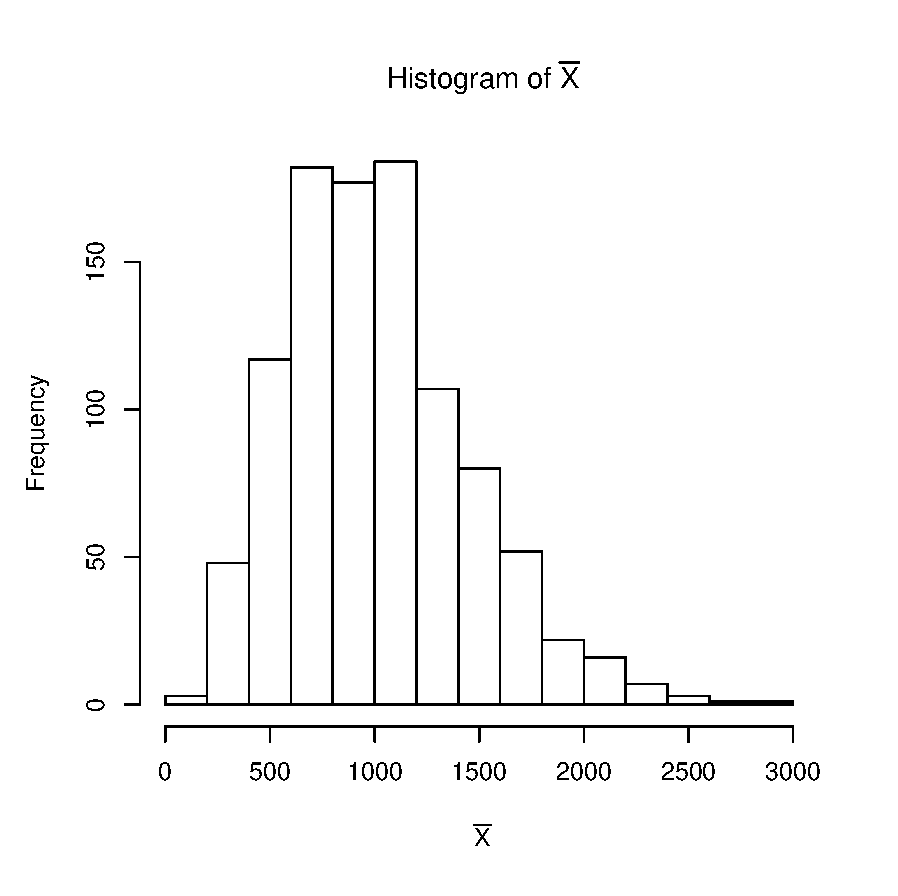
\includegraphics[width=0.5\textwidth, trim = 0.0cm 0.5cm 0.3cm 0.5cm, clip]{ExpHist5}
&&
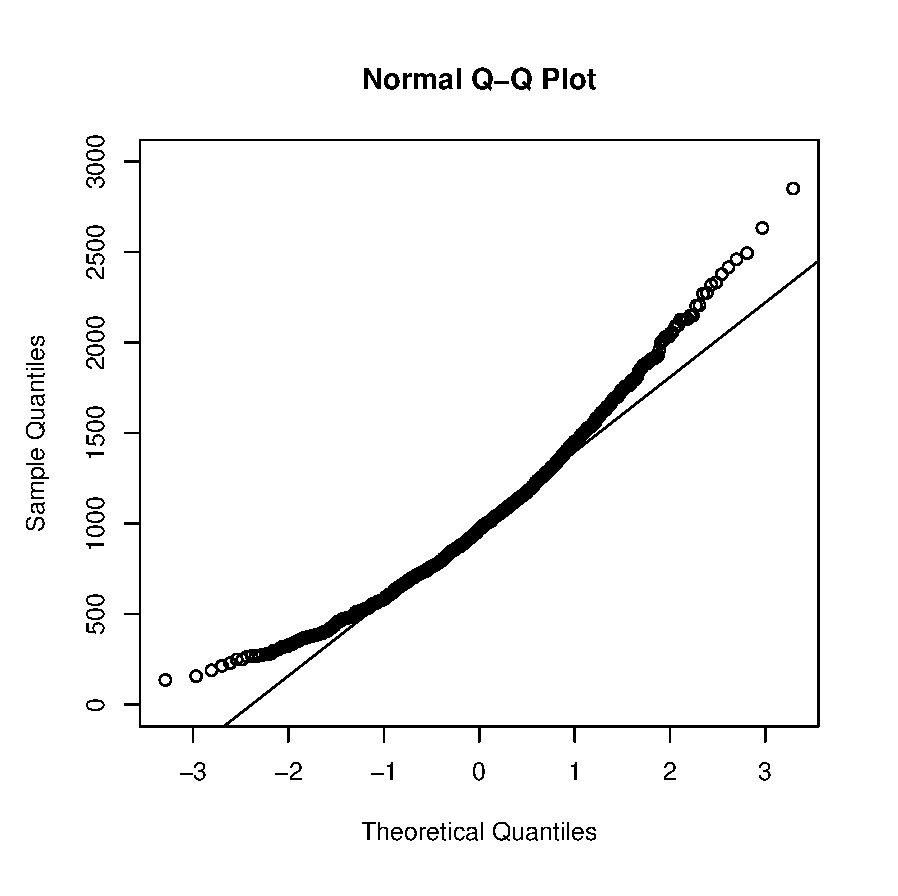
\includegraphics[width=0.5\textwidth, trim = 0.0cm 0.5cm 0.3cm 0.5cm, clip]{ExpNorm5}
\end{tabular}
\end{adjustwidth}

\end{frame}

%
\subsection{Example: Exponential Data}
\begin{frame}{\bf \tcb{Example: Exponential Data}}

$X \sim \text{Exponential}(\lambda=0.001)$ with $\boxed{n=10}$.

\begin{adjustwidth}{-0.2cm}{}
\begin{tabular}{c@{}c@{}c}
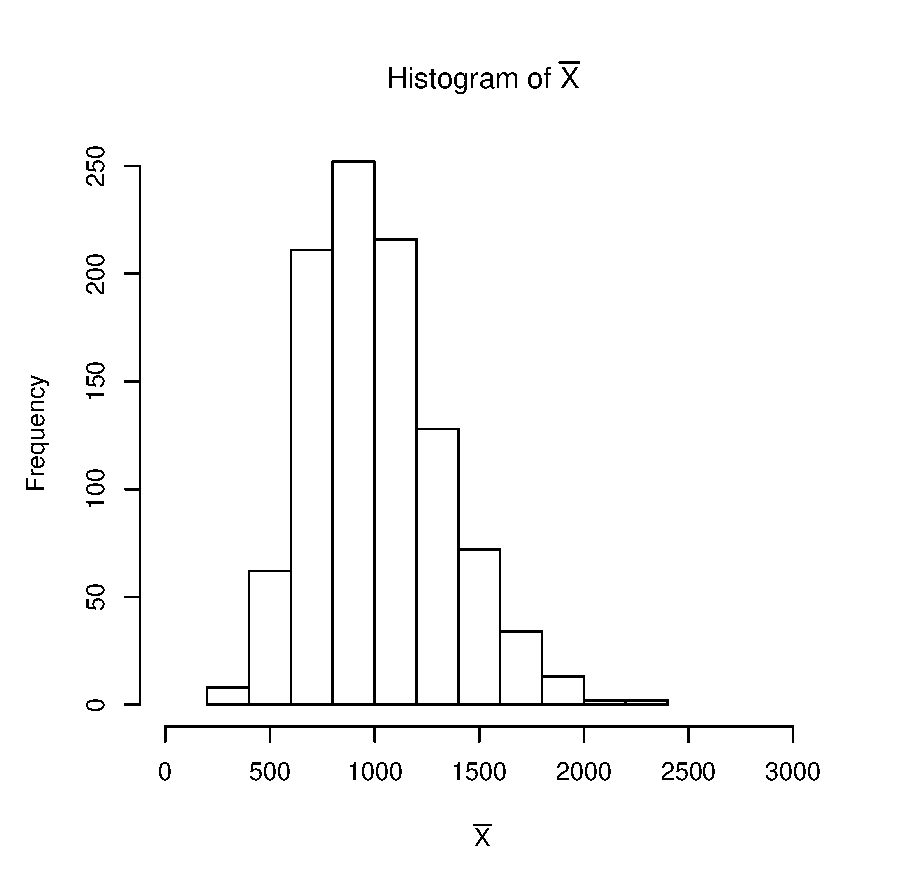
\includegraphics[width=0.5\textwidth, trim = 0.0cm 0.5cm 0.3cm 0.5cm, clip]{ExpHist10}
&&
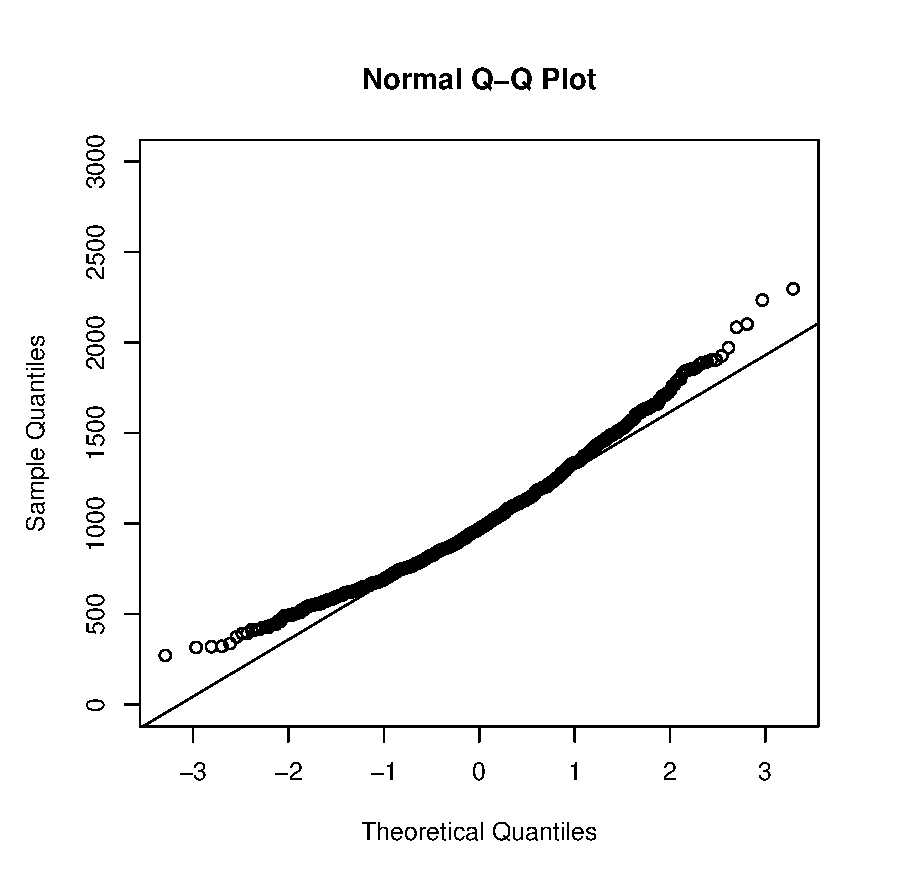
\includegraphics[width=0.5\textwidth, trim = 0.0cm 0.5cm 0.3cm 0.5cm, clip]{ExpNorm10}
\end{tabular}
\end{adjustwidth}

\end{frame}


\subsection{Example: Exponential Data}
\begin{frame}{\bf \tcb{Example: Exponential Data}}

$X \sim \text{Exponential}(\lambda=0.001)$ with $\boxed{n=30}$.

\begin{adjustwidth}{-0.2cm}{}
\begin{tabular}{c@{}c@{}c}
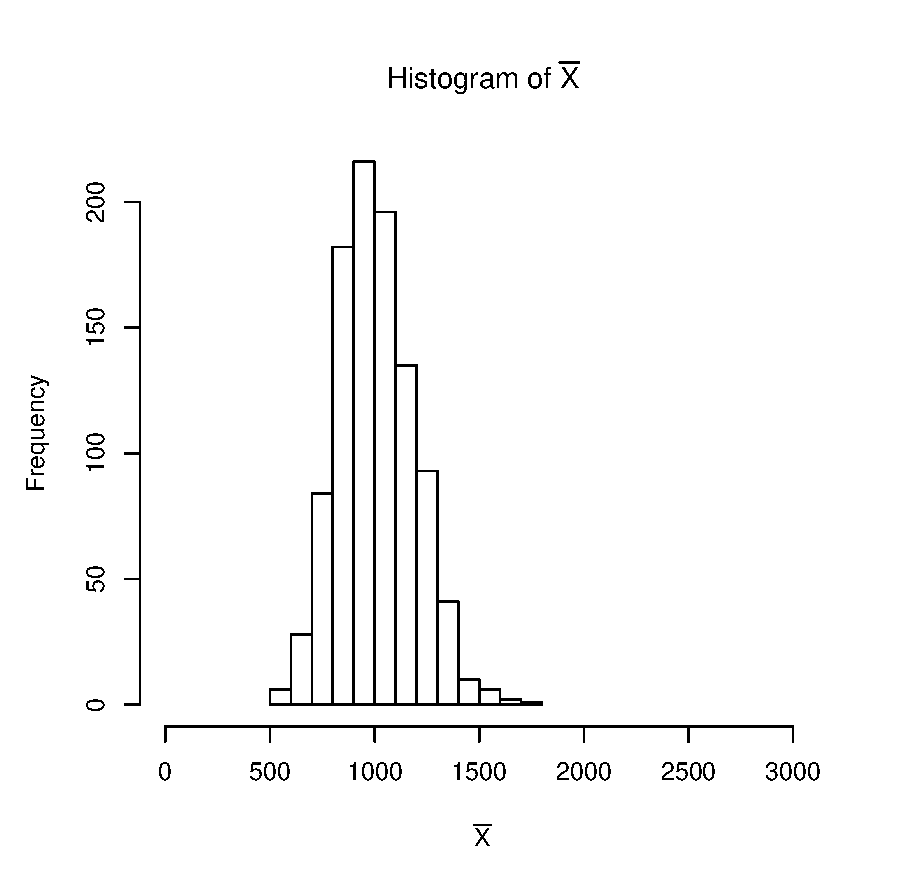
\includegraphics[width=0.5\textwidth, trim = 0.0cm 0.5cm 0.3cm 0.5cm, clip]{ExpHist30}
&&
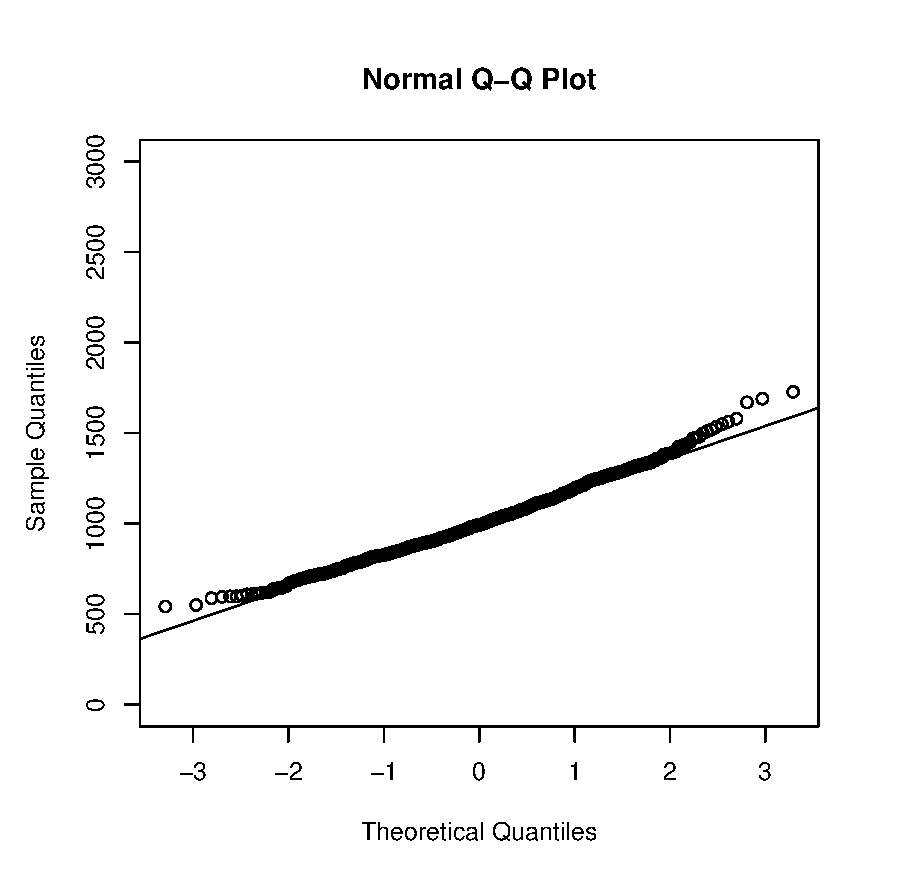
\includegraphics[width=0.5\textwidth, trim = 0.0cm 0.5cm 0.3cm 0.5cm, clip]{ExpNorm30}
\end{tabular}
\end{adjustwidth}

\end{frame}



\subsection{Example: Exponential Data}
\begin{frame}{\bf \tcb{Example: Exponential Data}}

$X \sim \text{Exponential}(\lambda=0.001)$ with $\boxed{n=60}$.

\begin{adjustwidth}{-0.2cm}{}
\begin{tabular}{c@{}c@{}c}
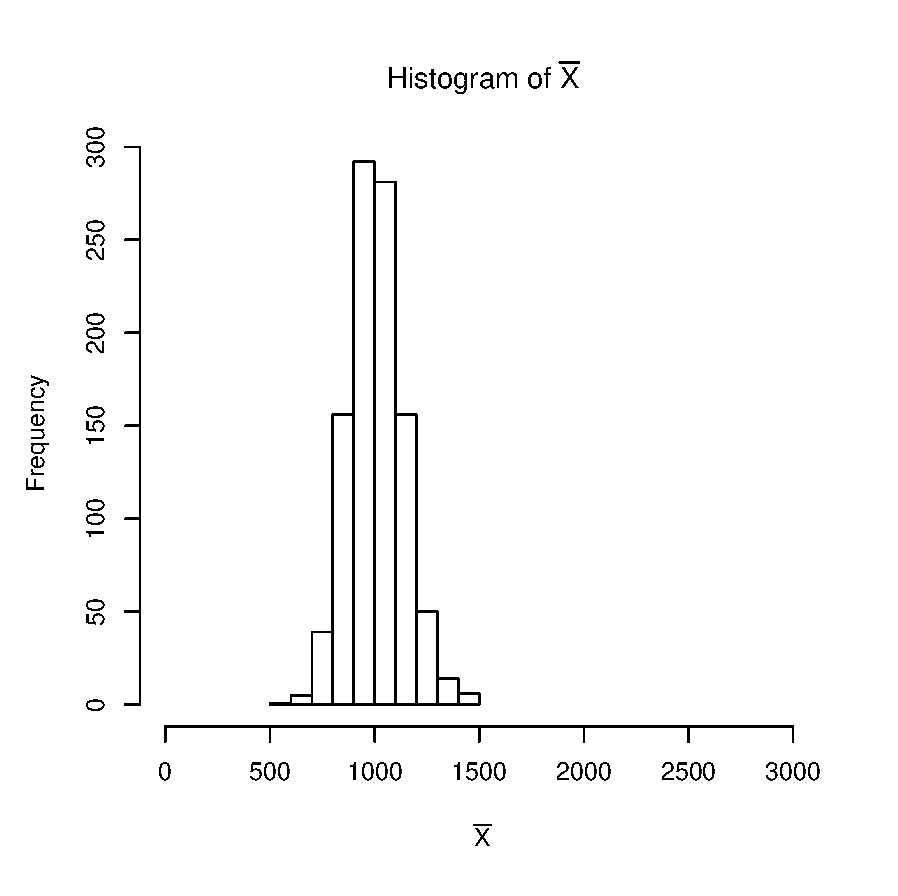
\includegraphics[width=0.5\textwidth, trim = 0.0cm 0.5cm 0.3cm 0.5cm, clip]{ExpHist60}
&&
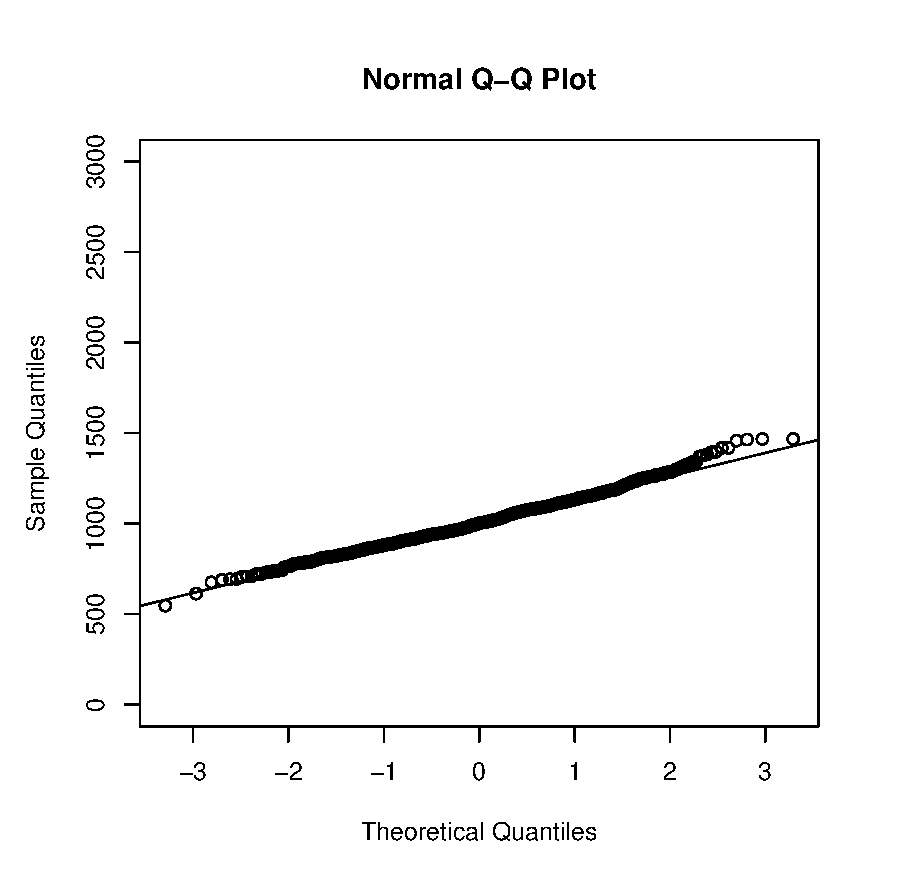
\includegraphics[width=0.5\textwidth, trim = 0.0cm 0.5cm 0.3cm 0.5cm, clip]{ExpNorm60}
\end{tabular}
\end{adjustwidth}

\end{frame}


\subsection{R Code}
\begin{frame}{\bf \tcb{R Code}}

Code for carrying out simulation:\\[0.4cm]

\begin{tabular}{|l|}
\hline
\texttt{n = 10\quad\# sample size}\\[0.3cm]
\texttt{set.seed(142981)}\\[0.3cm]
\texttt{simreps = 1000 \quad\# simulation replicates}\\
\texttt{\phantom{simreps = 1000} \quad\# (just needs to be a big number)}\\
\texttt{xbar = rep(0, simreps)}\\[0.3cm]
\texttt{for(i in 1:simreps)\{}\\
\texttt{\qquad xbar[i] = mean(rexp(n, rate=0.001))}\\
\texttt{\}}\\[0.3cm]
\texttt{hist(xbar, xlim=c(0,3000))}\\[0.3cm]
\texttt{qqnorm(xbar, ylim=c(0,3000));qqline(xbar)}\\
\hline
\multicolumn{1}{c}{}\\[0.0cm]
\end{tabular}

\end{frame}





\end{document} 